% =============================================================================
% Reporting Orchestrator Agent — Technical Documentation
% Version 1.0 | July 2026
% =============================================================================
\documentclass[12pt,a4paper]{article}

% ─── PACKAGES ───────────────────────────────
\usepackage[utf8]{inputenc}
\usepackage[T1]{fontenc}
\usepackage{geometry}
\usepackage{graphicx}
\usepackage{hyperref}
\usepackage{listings}
\usepackage{xcolor}
\usepackage{tikz}
\usepackage{pgfplots}
\usepackage{booktabs}
\usepackage{longtable}
\usepackage{tabularx}
\usepackage{enumitem}
\usepackage{fancyhdr}
\usepackage{titlesec}
\usepackage{tocloft}
\usepackage{amsmath}
\usepackage{mdframed}
\usepackage{float}
\usepackage{subcaption}
\usepackage{algorithm}
\usepackage{algpseudocode}
\usepackage{parskip}
\usepackage{multicol}
\usepackage{lmodern}

\usetikzlibrary{shapes.geometric, arrows.meta, positioning, fit, calc, backgrounds}
\pgfplotsset{compat=1.18}

% ─── PAGE GEOMETRY ──────────────────────────
\geometry{
  top=2.5cm,
  bottom=2.5cm,
  left=2.5cm,
  right=2.5cm
}

% ─── COLORS ─────────────────────────────────
\definecolor{apilayer}{RGB}{66,133,244}
\definecolor{logiclayer}{RGB}{52,168,83}
\definecolor{ailayer}{RGB}{154,109,218}
\definecolor{storagelayer}{RGB}{251,139,35}
\definecolor{infralayer}{RGB}{128,128,128}
\definecolor{uilayer}{RGB}{234,67,53}
\definecolor{codebg}{RGB}{245,245,245}
\definecolor{codeframe}{RGB}{200,200,200}
\definecolor{codegreen}{RGB}{40,120,40}
\definecolor{codeorange}{RGB}{200,100,0}
\definecolor{accentblue}{RGB}{30,90,180}
\definecolor{titlegray}{RGB}{60,60,60}
\definecolor{sectioncolor}{RGB}{30,90,180}

% ─── CODE LISTINGS ──────────────────────────
\lstset{
  backgroundcolor=\color{codebg},
  basicstyle=\ttfamily\small,
  breaklines=true,
  captionpos=b,
  commentstyle=\color{codegreen},
  keywordstyle=\color{accentblue}\bfseries,
  stringstyle=\color{codeorange},
  numberstyle=\tiny\color{gray},
  numbers=left,
  frame=single,
  rulecolor=\color{codeframe},
  tabsize=4,
  showstringspaces=false,
  xleftmargin=1.5em,
  framexleftmargin=1em,
  aboveskip=1em,
  belowskip=1em,
}

% ─── HEADERS & FOOTERS ─────────────────────
\pagestyle{fancy}
\fancyhf{}
\fancyhead[L]{\small\textcolor{titlegray}{Reporting Orchestrator Agent}}
\fancyhead[R]{\small\textcolor{titlegray}{Technical Documentation v1.0}}
\fancyfoot[C]{\thepage}
\fancyfoot[R]{\small\textcolor{titlegray}{Confidential}}
\renewcommand{\headrulewidth}{0.4pt}
\renewcommand{\footrulewidth}{0.2pt}

% ─── SECTION STYLING ───────────────────────
\titleformat{\section}
  {\Large\bfseries\color{sectioncolor}}
  {\thesection}{1em}{}[\vspace{-0.5em}\rule{\textwidth}{0.4pt}]

\titleformat{\subsection}
  {\large\bfseries\color{titlegray}}
  {\thesubsection}{1em}{}

\titleformat{\subsubsection}
  {\normalsize\bfseries\color{titlegray}}
  {\thesubsubsection}{1em}{}

% ─── HYPERREF SETUP ─────────────────────────
\hypersetup{
  colorlinks=true,
  linkcolor=accentblue,
  urlcolor=accentblue,
  citecolor=accentblue,
  pdfauthor={Rishabh Saklani},
  pdftitle={Reporting Orchestrator Agent — Technical Documentation},
  pdfsubject={Enterprise AI-Powered Workday Report Migration},
}

% ─── INFO / WARNING BOXES ──────────────────
\newmdenv[
  backgroundcolor=apilayer!8,
  linecolor=apilayer,
  linewidth=1.5pt,
  leftmargin=0pt,
  rightmargin=0pt,
  innertopmargin=10pt,
  innerbottommargin=10pt,
  innerleftmargin=12pt,
  innerrightmargin=12pt,
  roundcorner=4pt,
  skipabove=10pt,
  skipbelow=10pt
]{infobox}

\newmdenv[
  backgroundcolor=storagelayer!10,
  linecolor=storagelayer,
  linewidth=1.5pt,
  leftmargin=0pt,
  rightmargin=0pt,
  innertopmargin=10pt,
  innerbottommargin=10pt,
  innerleftmargin=12pt,
  innerrightmargin=12pt,
  roundcorner=4pt,
  skipabove=10pt,
  skipbelow=10pt
]{warningbox}

\newmdenv[
  backgroundcolor=logiclayer!8,
  linecolor=logiclayer,
  linewidth=1.5pt,
  leftmargin=0pt,
  rightmargin=0pt,
  innertopmargin=10pt,
  innerbottommargin=10pt,
  innerleftmargin=12pt,
  innerrightmargin=12pt,
  roundcorner=4pt,
  skipabove=10pt,
  skipbelow=10pt
]{successbox}

% ─── TOC STYLING ───────────────────────────
\renewcommand{\cftsecleader}{\cftdotfill{\cftdotsep}}

% ─── LIST OF LISTINGS ──────────────────────
\renewcommand{\lstlistlistingname}{List of Code Listings}

% =============================================================================
% DOCUMENT BEGIN
% =============================================================================
\begin{document}

% =============================================================================
% COVER PAGE
% =============================================================================
\begin{titlepage}
\centering
\vspace*{2cm}

{\Huge\bfseries\textcolor{sectioncolor}{Reporting Orchestrator Agent}}\\[0.8cm]
{\Large\textcolor{titlegray}{AI-Powered Workday Report Migration Platform}}\\[1.5cm]

\rule{0.8\textwidth}{1pt}\\[1.2cm]

{\large\textbf{Technical Documentation}}\\[0.5cm]
{\large Version 1.0}\\[2cm]

\begin{tabular}{rl}
  \textbf{Author:}        & Rishabh Saklani \\[0.3cm]
  \textbf{Role:}           & Software Developer \\[0.3cm]
  \textbf{Organization:}   & Accenture \\[0.3cm]
  \textbf{Date:}           & July 23, 2026 \\[0.3cm]
  \textbf{Version:}        & v1.0 \\[0.3cm]
\end{tabular}

\vfill

\rule{0.8\textwidth}{0.4pt}\\[0.5cm]
{\small\textcolor{titlegray}{\textbf{CONFIDENTIAL} --- For internal use only}}

\end{titlepage}

% =============================================================================
% TABLE OF CONTENTS
% =============================================================================
\newpage
\tableofcontents
\newpage
\listoffigures
\listoftables
\lstlistoflistings
\newpage

% =============================================================================
% SECTION 1: EXECUTIVE SUMMARY
% =============================================================================
\section{Executive Summary}
\label{sec:executive-summary}

\subsection{Project Overview}
\label{subsec:project-overview}

The \textbf{Reporting Orchestrator Agent} is an enterprise-grade, AI-powered browser automation platform designed to streamline the migration of Workday Custom Reports and Dashboards between tenant environments. It combines a natural-language report discovery engine (powered by BM25 retrieval and LLM re-ranking) with config-driven Playwright browser automation to eliminate the manual, error-prone process of navigating the Workday UI to create Configuration Packages, select reports, and export definitions.

The platform is built for \textbf{Workday implementation consultants and migration teams} at Accenture who need to migrate hundreds of custom reports across Workday tenants during implementation projects. It replaces a process that previously required hours of repetitive manual clicks with a single automated workflow that completes in minutes.

The system is delivered as both a Python web application (FastAPI + vanilla HTML/CSS/JS) and a standalone Windows \texttt{.exe} executable, making it accessible to non-technical users without requiring Python installation.

\subsection{Key Outcomes \& Impact}
\label{subsec:key-outcomes}

\begin{itemize}[leftmargin=2em]
  \item \textbf{Time Reduction:} Migration of 50+ reports reduced from 4--6 hours of manual work to under 15 minutes of automated execution.
  \item \textbf{Error Elimination:} Config-driven step execution eliminates human errors in report selection, package naming, and migration triggers.
  \item \textbf{AI-Powered Discovery:} Natural-language search over 11,600+ Workday reports with LLM-scored relevance ranking replaces manual catalog browsing.
  \item \textbf{Parallel Execution:} Migration and Export agents run concurrently in isolated browser contexts via \texttt{asyncio.gather}, halving total execution time.
  \item \textbf{Zero-Install Distribution:} PyInstaller-bundled \texttt{.exe} with auto-generated \texttt{.env} template enables one-click deployment to any Windows machine.
\end{itemize}

% =============================================================================
% SECTION 2: PROJECT BACKGROUND
% =============================================================================
\section{Project Background}
\label{sec:project-background}

\subsection{Problem Statement}
\label{subsec:problem-statement}

Workday implementation projects routinely require migrating custom reports and dashboards between tenant environments (e.g., from a development tenant to a production tenant). The standard Workday process involves:

\begin{enumerate}[leftmargin=2em]
  \item Navigating to the \textit{Create Configuration Package} task in Workday.
  \item Naming the package with a specific naming convention.
  \item Selecting the implementation type (Custom Reports or Custom Dashboards with Tabs).
  \item Filtering and individually selecting each report from a grid containing thousands of entries.
  \item Clicking \textit{Migrate} and waiting for the package to generate.
  \item Optionally exporting report definitions as Excel files for documentation.
\end{enumerate}

For a typical engagement with 50--100 reports, this process takes \textbf{4--6 hours} of tedious, repetitive clicking. Key pain points include:

\begin{itemize}[leftmargin=2em]
  \item \textbf{Manual Report Identification:} Consultants must know the exact report names. With 11,600+ custom reports in a tenant, finding the right ones is time-consuming.
  \item \textbf{Repetitive UI Navigation:} Each report requires filtering the grid, scrolling, ticking a checkbox, and clearing the filter --- repeated dozens of times.
  \item \textbf{Human Error Risk:} Misspelled names, missed reports, or incorrect package configurations lead to failed migrations that must be restarted.
  \item \textbf{No Parallelism:} Migration and export must be done sequentially in the browser, doubling the total time.
  \item \textbf{Knowledge Gap:} New team members struggle to identify which reports are relevant for a given industry or use case.
\end{itemize}

% =============================================================================
% SECTION 3: PREREQUISITES & DEPENDENCIES
% =============================================================================
\section{Prerequisites \& Dependencies}
\label{sec:prerequisites}

\subsection{System Requirements}
\label{subsec:system-requirements}

\begin{table}[H]
\centering
\caption{System Requirements}
\label{tab:system-requirements}
\begin{tabularx}{\textwidth}{l X X}
\toprule
\textbf{Component} & \textbf{Minimum} & \textbf{Recommended} \\
\midrule
Operating System & Windows 10 (64-bit) & Windows 11 \\
RAM & 4 GB & 8 GB \\
CPU & Dual-core 2.0 GHz & Quad-core 3.0 GHz \\
Storage & 500 MB free & 1 GB free \\
Network & Broadband internet & Low-latency connection \\
Browser & Chromium (auto-installed) & Google Chrome (latest) \\
Display & 1280$\times$720 & 1440$\times$900 or higher \\
\bottomrule
\end{tabularx}
\end{table}

\subsection{Software Prerequisites}
\label{subsec:software-prerequisites}

\begin{table}[H]
\centering
\caption{Software Dependencies}
\label{tab:software-dependencies}
\begin{tabularx}{\textwidth}{l l X l}
\toprule
\textbf{Software} & \textbf{Version} & \textbf{Purpose} & \textbf{Required} \\
\midrule
Python & $\geq$ 3.11 & Runtime environment & Yes* \\
Playwright & $\geq$ 1.50.0 & Browser automation engine & Yes \\
FastAPI & $\geq$ 0.100.0 & Web server framework & Yes \\
Uvicorn & $\geq$ 0.23.0 & ASGI server & Yes \\
OpenAI SDK & $\geq$ 1.0.0 & LLM API client (Groq) & Yes \\
python-dotenv & $\geq$ 1.0.0 & Environment variable loader & Yes \\
Rich & $\geq$ 13.0.0 & Terminal formatting (CLI) & Yes \\
Pandas & $\geq$ 2.0.0 & Data processing & Yes \\
Requests & $\geq$ 2.25.0 & HTTP client for RaaS sync & Yes \\
PyInstaller & $\geq$ 6.0.0 & Executable packaging & Optional \\
\bottomrule
\end{tabularx}
\end{table}

\begin{infobox}
\textbf{Note:} When using the standalone \texttt{.exe} build, Python is \textbf{not} required on the target machine. All dependencies are bundled into the executable.
\end{infobox}

\subsection{Account \& Access Prerequisites}
\label{subsec:account-prerequisites}

\begin{table}[H]
\centering
\caption{Environment Variables}
\label{tab:env-vars}
\begin{tabularx}{\textwidth}{l X l}
\toprule
\textbf{Variable} & \textbf{Description} & \textbf{Required} \\
\midrule
\texttt{OPENAI\_API\_KEY} & Groq Cloud API key for LLM scoring & For AI search \\
\texttt{OPENAI\_BASE\_URL} & LLM API endpoint (Groq) & For AI search \\
\texttt{MODEL\_NAME} & LLM model identifier & For AI search \\
\texttt{WD\_USER} & Workday tenant login username & Yes \\
\texttt{WD\_PASS} & Workday tenant login password & Yes \\
\texttt{WORKDAY\_RAAS\_URL} & Workday RaaS endpoint for catalog sync & For live sync \\
\texttt{WORKDAY\_ISU\_USERNAME} & ISU service account username & For live sync \\
\texttt{WORKDAY\_ISU\_PASSWORD} & ISU service account password & For live sync \\
\texttt{BM25\_TOP\_N} & Number of BM25 candidates (default: 30) & No \\
\texttt{LLM\_TOP\_K} & Number of final LLM results (default: 5) & No \\
\bottomrule
\end{tabularx}
\end{table}

\subsection{Knowledge Prerequisites}
\label{subsec:knowledge-prerequisites}

\begin{itemize}[leftmargin=2em]
  \item \textbf{Users:} Basic familiarity with Workday tenant navigation and report names.
  \item \textbf{Administrators:} Understanding of Workday Configuration Packages and Implementation Types.
  \item \textbf{Developers:} Python 3.11+, Playwright, FastAPI, and basic understanding of BM25/LLM concepts for maintenance.
\end{itemize}

\subsection{Installation Dependencies}
\label{subsec:installation-dependencies}

\begin{lstlisting}[language=bash, caption={Install all dependencies}, label={lst:install-deps}]
pip install -r requirements.txt
playwright install chromium
\end{lstlisting}

\begin{lstlisting}[caption={requirements.txt}, label={lst:requirements-txt}]
# Core automation
playwright>=1.50.0

# Report Discovery Agent
fastapi>=0.100.0
uvicorn[standard]>=0.23.0
openai>=1.0.0
python-dotenv>=1.0.0
rich>=13.0.0
pandas>=2.0.0
requests>=2.25.0

# Packaging
pyinstaller>=6.0.0
\end{lstlisting}

% =============================================================================
% SECTION 4: SYSTEM ARCHITECTURE
% =============================================================================
\section{System Architecture}
\label{sec:architecture}

\subsection{Architecture Overview}
\label{subsec:arch-overview}

The Reporting Orchestrator Agent follows a \textbf{layered architecture} with clear separation of concerns:

\begin{itemize}[leftmargin=2em]
  \item \textbf{Presentation Layer:} A single-page web application (HTML/CSS/JS) served by FastAPI, with SSE (Server-Sent Events) for real-time progress streaming.
  \item \textbf{API Layer:} FastAPI REST endpoints for workflow launch, cancellation, pause/resume, and status queries.
  \item \textbf{Orchestration Layer:} A background thread that manages the workflow lifecycle, spawning Playwright browser contexts and coordinating agent execution.
  \item \textbf{Agent Layer:} Config-driven step executors that translate declarative JSON step definitions into Playwright browser actions.
  \item \textbf{AI Layer:} A two-stage retrieval pipeline (BM25 $\rightarrow$ LLM re-ranking) for natural-language report discovery.
  \item \textbf{Data Layer:} JSON catalog files, environment configuration, and file-based inter-process communication.
\end{itemize}

\subsection{Architecture Diagram}
\label{subsec:arch-diagram}

\begin{figure}[H]
\centering
\resizebox{0.95\textwidth}{!}{%
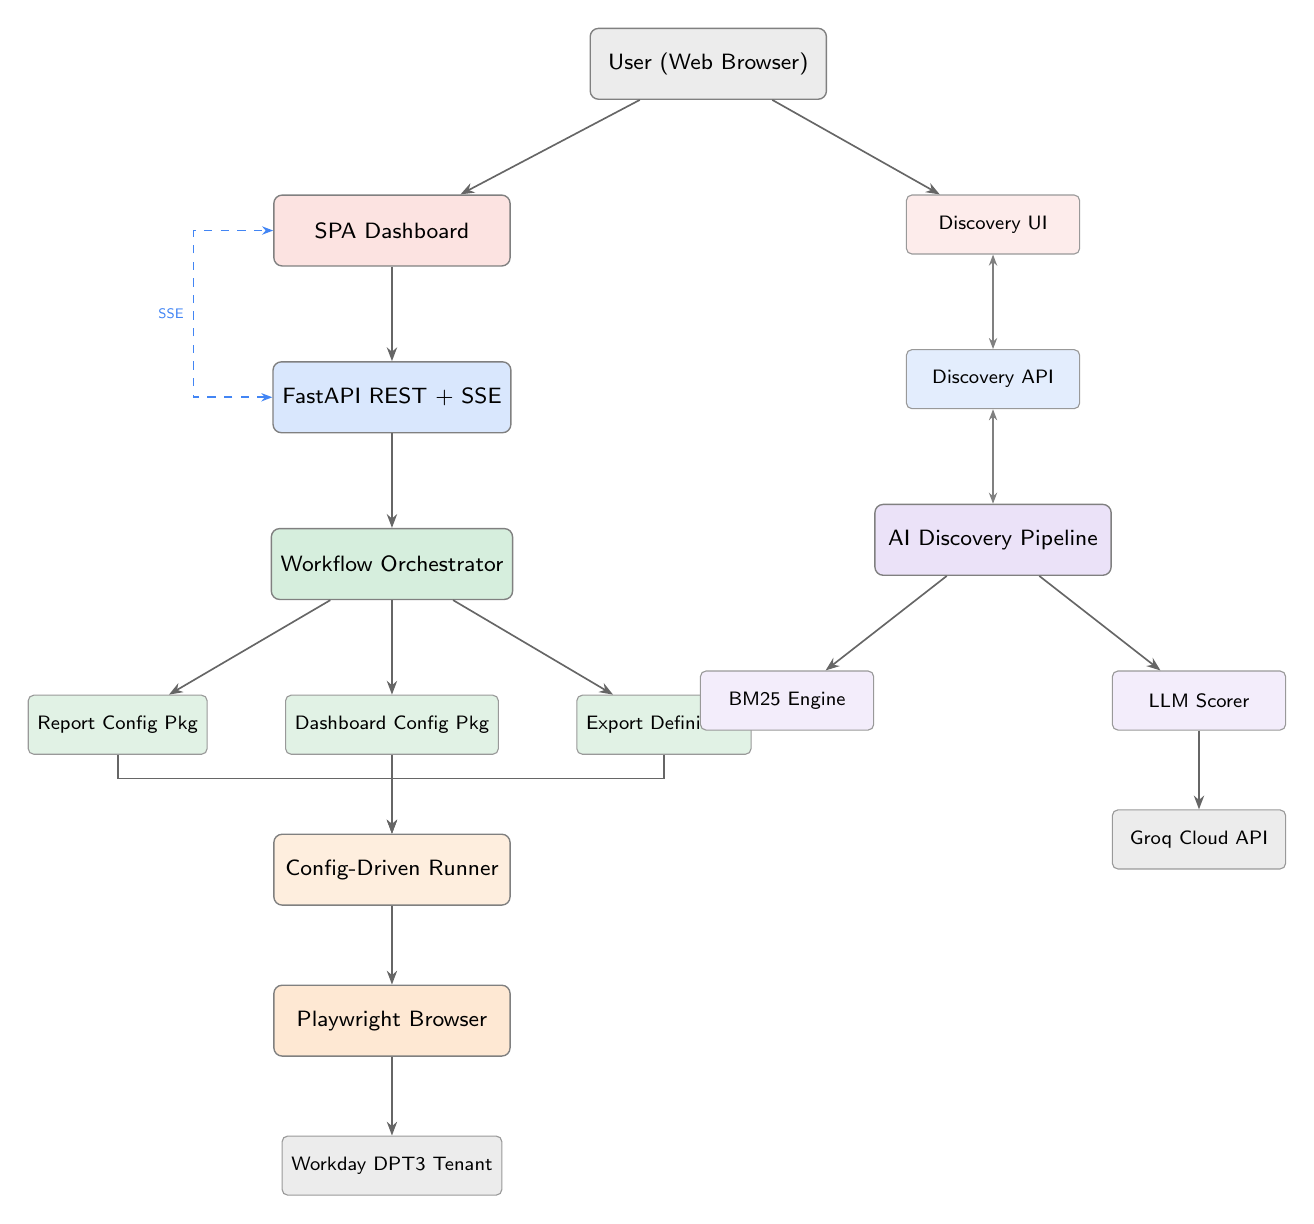
\begin{tikzpicture}[
  node distance=1cm and 1.2cm,
  box/.style={
    rectangle, rounded corners=3pt,
    minimum width=3cm, minimum height=0.9cm,
    text centered, draw=black!50, line width=0.5pt,
    font=\footnotesize\sffamily
  },
  smallbox/.style={
    rectangle, rounded corners=2pt,
    minimum width=2.2cm, minimum height=0.75cm,
    text centered, draw=black!40, line width=0.4pt,
    font=\scriptsize\sffamily
  },
  arrow/.style={-{Stealth[length=5pt]}, semithick, draw=black!60},
  darrow/.style={
    {Stealth[length=4pt]}-{Stealth[length=4pt]},
    semithick, draw=black!50
  }
]

% ── User Layer ──
\node[box, fill=infralayer!15] (user) {User (Web Browser)};

% ── Presentation Layer (side by side) ──
\node[box, fill=uilayer!15, below left=1.2cm and 1cm of user] (spa) {SPA Dashboard};
\node[smallbox, fill=uilayer!10, below right=1.2cm and 1cm of user] (discovery_ui) {Discovery UI};

% ── API Layer ──
\node[box, fill=apilayer!20, below=1.2cm of spa] (api) {FastAPI REST + SSE};
\node[smallbox, fill=apilayer!15, below=1.2cm of discovery_ui] (disc_api) {Discovery API};

% ── Orchestration + AI side by side ──
\node[box, fill=logiclayer!20, below=1.2cm of api] (orchestrator) {Workflow Orchestrator};
\node[box, fill=ailayer!20, below=1.2cm of disc_api] (ai_pipeline) {AI Discovery Pipeline};

% ── Agent Layer (stacked vertically under orchestrator) ──
\node[smallbox, fill=logiclayer!15, below left=1.2cm and 0.8cm of orchestrator] (migration) {Report Config Pkg};
\node[smallbox, fill=logiclayer!15, below=1.2cm of orchestrator] (dashboard) {Dashboard Config Pkg};
\node[smallbox, fill=logiclayer!15, below right=1.2cm and 0.8cm of orchestrator] (export) {Export Definitions};

% ── AI sub-components ──
\node[smallbox, fill=ailayer!12, below left=1.2cm and 0cm of ai_pipeline] (bm25) {BM25 Engine};
\node[smallbox, fill=ailayer!12, below right=1.2cm and 0cm of ai_pipeline] (llm) {LLM Scorer};

% ── Runner Engine ──
\node[box, fill=storagelayer!15, below=1cm of dashboard] (runner) {Config-Driven Runner};

% ── External ──
\node[smallbox, fill=infralayer!15, below=1cm of llm] (groq) {Groq Cloud API};
\node[box, fill=storagelayer!20, below=1cm of runner] (playwright) {Playwright Browser};
\node[smallbox, fill=infralayer!15, below=1cm of playwright] (workday) {Workday DPT3 Tenant};

% ── Arrows: User down ──
\draw[arrow] (user) -- (spa);
\draw[arrow] (user) -- (discovery_ui);

% ── Arrows: Presentation to API ──
\draw[arrow] (spa) -- (api);
\draw[darrow] (discovery_ui) -- (disc_api);

% ── Arrows: API to Logic ──
\draw[arrow] (api) -- (orchestrator);
\draw[darrow] (disc_api) -- (ai_pipeline);

% ── Arrows: Orchestrator to Agents ──
\draw[arrow] (orchestrator) -- (migration);
\draw[arrow] (orchestrator) -- (dashboard);
\draw[arrow] (orchestrator) -- (export);

% ── Arrows: Agents to Runner ──
\draw[arrow] (migration.south) -- ++(0,-0.3) -| (runner);
\draw[arrow] (dashboard) -- (runner);
\draw[arrow] (export.south) -- ++(0,-0.3) -| (runner);

% ── Arrows: AI sub-components ──
\draw[arrow] (ai_pipeline) -- (bm25);
\draw[arrow] (ai_pipeline) -- (llm);
\draw[arrow] (llm) -- (groq);

% ── Arrows: Runner to Browser ──
\draw[arrow] (runner) -- (playwright);
\draw[arrow] (playwright) -- (workday);

% ── SSE feedback arrow ──
\draw[darrow, dashed, draw=apilayer] (api.west) -- ++(-1,0) |- (spa.west)
  node[pos=0.25, left, font=\tiny\sffamily, text=apilayer] {SSE};

\end{tikzpicture}%
}% end resizebox
\caption{High-Level System Architecture}
\label{fig:architecture}
\end{figure}

\subsection{Component Breakdown}
\label{subsec:component-breakdown}

\subsubsection{Orchestrator Web UI (\texttt{orchestrator\_ui/server.py})}
\begin{itemize}[leftmargin=2em]
  \item \textbf{Purpose:} Serves the SPA dashboard, exposes REST API endpoints, and manages SSE event streaming for real-time progress updates.
  \item \textbf{Inputs:} Workflow selection, credentials, report/dashboard names, package name.
  \item \textbf{Outputs:} SSE event stream (\texttt{agent\_start}, \texttt{step}, \texttt{agent\_done}, \texttt{all\_done}), JSON API responses.
  \item \textbf{Technology:} FastAPI, Uvicorn, Server-Sent Events.
\end{itemize}

\subsubsection{Config-Driven Runner (\texttt{runner.py})}
\begin{itemize}[leftmargin=2em]
  \item \textbf{Purpose:} Executes a declarative JSON configuration of browser steps against a Playwright browser context. Supports 15+ action types.
  \item \textbf{Inputs:} JSON config dict with \texttt{steps[]} array, Playwright \texttt{BrowserContext}.
  \item \textbf{Outputs:} Exit code (0=success, 1=failure), error message string.
  \item \textbf{Technology:} Playwright (sync and async APIs).
\end{itemize}

\subsubsection{Report Config Package Agent (\texttt{run\_agent.py})}
\begin{itemize}[leftmargin=2em]
  \item \textbf{Purpose:} Builds the step configuration for creating a Workday Configuration Package with Custom Reports implementation type.
  \item \textbf{Inputs:} Industry name, list of report names.
  \item \textbf{Outputs:} JSON config dict consumed by \texttt{runner.py}.
\end{itemize}

\subsubsection{Dashboard Config Package Agent (\texttt{run\_dashboard\_agent.py})}
\begin{itemize}[leftmargin=2em]
  \item \textbf{Purpose:} Analogous to the Report agent but for Custom Dashboards with Tabs implementation type.
  \item \textbf{Inputs:} Industry name, list of dashboard names.
  \item \textbf{Outputs:} JSON config dict consumed by \texttt{runner.py}.
\end{itemize}

\subsubsection{Export Definitions Agent (\texttt{run\_export.py})}
\begin{itemize}[leftmargin=2em]
  \item \textbf{Purpose:} Navigates to each report in Workday and downloads its definition as an Excel file via the ``Export to Excel'' action.
  \item \textbf{Inputs:} List of report names.
  \item \textbf{Outputs:} Excel files saved to \texttt{exported\_reports/} directory.
\end{itemize}

\subsubsection{Report Discovery Agent (\texttt{Workday\_Report\_Discovery\_Agent/})}
\begin{itemize}[leftmargin=2em]
  \item \textbf{Purpose:} AI-powered search over 11,600+ Workday custom reports using a two-stage BM25 $\rightarrow$ LLM pipeline.
  \item \textbf{Inputs:} Natural-language user query.
  \item \textbf{Outputs:} Ranked list of reports with relevance scores, bands (High/Medium/Low), and explanations.
  \item \textbf{Technology:} Custom BM25 engine, OpenAI-compatible LLM via Groq Cloud, FastAPI sub-application.
\end{itemize}

\subsection{Data Flow Diagram}
\label{subsec:data-flow}

\begin{figure}[H]
\centering
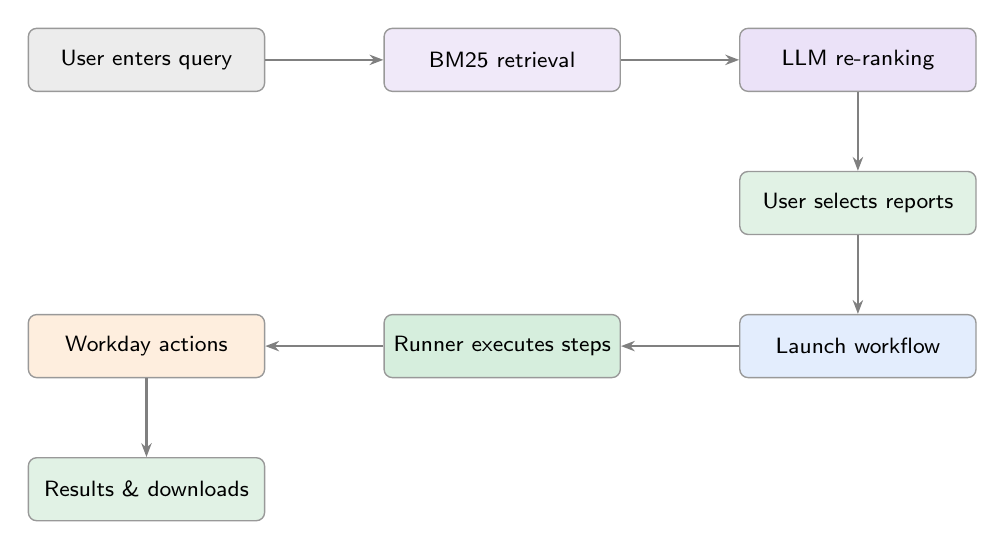
\begin{tikzpicture}[
  node distance=1cm and 1.5cm,
  step/.style={
    rectangle, rounded corners=3pt,
    minimum width=3cm, minimum height=0.8cm,
    text centered, draw=black!40, line width=0.5pt,
    font=\footnotesize\sffamily, fill=#1
  },
  arrow/.style={-{Stealth[length=5pt]}, thick, draw=black!50}
]

\node[step=infralayer!15] (input) {User enters query};
\node[step=ailayer!15, right=of input] (bm25) {BM25 retrieval};
\node[step=ailayer!20, right=of bm25] (llm) {LLM re-ranking};
\node[step=logiclayer!15, below=of llm] (select) {User selects reports};
\node[step=apilayer!15, below=of select] (launch) {Launch workflow};
\node[step=logiclayer!20, left=of launch] (runner) {Runner executes steps};
\node[step=storagelayer!15, left=of runner] (workday) {Workday actions};
\node[step=logiclayer!15, below=of workday] (result) {Results \& downloads};

\draw[arrow] (input) -- (bm25);
\draw[arrow] (bm25) -- (llm);
\draw[arrow] (llm) -- (select);
\draw[arrow] (select) -- (launch);
\draw[arrow] (launch) -- (runner);
\draw[arrow] (runner) -- (workday);
\draw[arrow] (workday) -- (result);

\end{tikzpicture}
\caption{End-to-End Data Flow}
\label{fig:data-flow}
\end{figure}

\subsection{API Architecture}
\label{subsec:api-architecture}

\begin{table}[H]
\centering
\caption{Orchestrator REST API Endpoints}
\label{tab:api-endpoints}
\begin{tabularx}{\textwidth}{l l X l}
\toprule
\textbf{Endpoint} & \textbf{Method} & \textbf{Purpose} & \textbf{Auth} \\
\midrule
\texttt{/} & GET & Serve SPA dashboard HTML & None \\
\texttt{/api/health} & GET & Health check & None \\
\texttt{/api/env-status} & GET & Check configured env vars & None \\
\texttt{/api/launch} & POST & Launch a workflow & Body \\
\texttt{/api/cancel} & POST & Force-cancel running workflow & None \\
\texttt{/api/force-reset} & POST & Reset stuck run state & None \\
\texttt{/api/status} & GET & Poll current run status & None \\
\texttt{/api/events} & GET & SSE event stream & None \\
\texttt{/api/pause-resolve} & POST & Resume paused workflow & None \\
\texttt{/api/start-discovery} & POST & No-op (backward compat) & None \\
\texttt{/api/discovery-reports} & GET & Get confirmed report selection & None \\
\bottomrule
\end{tabularx}
\end{table}

\begin{table}[H]
\centering
\caption{Discovery Agent API Endpoints (mounted at \texttt{/discovery})}
\label{tab:discovery-api}
\begin{tabularx}{\textwidth}{l l X l}
\toprule
\textbf{Endpoint} & \textbf{Method} & \textbf{Purpose} & \textbf{Auth} \\
\midrule
\texttt{/api/search} & POST & Search reports with BM25 + LLM & None \\
\texttt{/api/sync} & POST & Sync catalog from Workday RaaS & None \\
\texttt{/api/stats} & GET & Catalog statistics & None \\
\texttt{/api/sync-status} & GET & Background sync status & None \\
\texttt{/api/confirm} & POST & Confirm report selection & None \\
\texttt{/api/selection} & GET & Get current selection & None \\
\bottomrule
\end{tabularx}
\end{table}

\subsection{Data Model}
\label{subsec:data-model}

The system uses file-based data storage rather than a traditional database:

\begin{lstlisting}[caption={Report Catalog JSON Schema (per entry)}, label={lst:report-schema}, language={}]
{
  "Report_Name": "Employee Termination Report",
  "Report_Type": "Custom",
  "Brief_Description": "Shows termination details...",
  "DS_Description": "All Workers data source",
  "Fields_Displayed_on_Report": "Employee ID, Name, ...",
  "Fields_Referenced_in_Report": "Termination Date, ..."
}
\end{lstlisting}

% =============================================================================
% SECTION 5: TECH STACK
% =============================================================================
\section{Tech Stack}
\label{sec:tech-stack}

\subsection{Technology Overview}
\label{subsec:tech-overview}

\begin{table}[H]
\centering
\caption{Technology Stack Summary}
\label{tab:tech-stack}
\begin{tabularx}{\textwidth}{l l l X}
\toprule
\textbf{Layer} & \textbf{Technology} & \textbf{Version} & \textbf{Purpose} \\
\midrule
Frontend & HTML/CSS/JS & ES6+ & Single-page dashboard UI \\
Backend & FastAPI & $\geq$0.100 & REST API + SSE server \\
Backend & Uvicorn & $\geq$0.23 & ASGI HTTP server \\
Automation & Playwright & $\geq$1.50 & Browser automation engine \\
AI/Search & BM25 (custom) & --- & First-stage keyword retrieval \\
AI/LLM & Groq Cloud & --- & LLM re-ranking via LLaMA 3.3 70B \\
AI/SDK & OpenAI Python & $\geq$1.0 & API client for Groq \\
NLP & Custom stemmer & --- & Suffix-stripping tokenizer \\
NLP & Synonym dict & --- & HR-domain query expansion \\
Data & JSON files & --- & Report catalog storage \\
Data & Pandas & $\geq$2.0 & Catalog data processing \\
HTTP & Requests & $\geq$2.25 & Workday RaaS sync \\
Config & python-dotenv & $\geq$1.0 & \texttt{.env} file loading \\
CLI & Rich & $\geq$13.0 & Terminal output formatting \\
Packaging & PyInstaller & $\geq$6.0 & Standalone \texttt{.exe} builder \\
\bottomrule
\end{tabularx}
\end{table}

\subsection{AI / LLM Stack}
\label{subsec:ai-stack}

\begin{itemize}[leftmargin=2em]
  \item \textbf{Model:} Meta LLaMA 3.3 70B Versatile, hosted on Groq Cloud.
  \item \textbf{API:} OpenAI-compatible REST API via \texttt{https://api.groq.com/openai/v1}.
  \item \textbf{Temperature:} 0.0 (deterministic scoring).
  \item \textbf{Max Tokens:} 8,192 per request.
  \item \textbf{Prompt Engineering:} Structured system prompt with metadata completeness penalties, relevance bands (High/Medium/Low), and mandatory JSON output format.
  \item \textbf{Retry Strategy:} Automatic retry with exponential backoff (5s $\rightarrow$ 15s $\rightarrow$ 30s) on HTTP 429 rate limit errors, with graceful BM25 fallback after 3 failures.
\end{itemize}

\subsection{Third-Party Integrations}
\label{subsec:third-party}

\begin{table}[H]
\centering
\caption{External Service Integrations}
\label{tab:integrations}
\begin{tabularx}{\textwidth}{l X l l l}
\toprule
\textbf{Service} & \textbf{Purpose} & \textbf{API Type} & \textbf{Tier} & \textbf{Limits} \\
\midrule
Groq Cloud & LLM inference & REST & Free & 100K TPD \\
Workday DPT3 & Target tenant & Web UI & Licensed & N/A \\
Workday RaaS & Catalog sync & REST/JSON & Licensed & N/A \\
\bottomrule
\end{tabularx}
\end{table}

% =============================================================================
% SECTION 6: PROJECT STRUCTURE
% =============================================================================
\section{Project Structure}
\label{sec:project-structure}

\subsection{Repository Structure}
\label{subsec:repo-structure}

\begin{lstlisting}[caption={Complete Project Tree}, label={lst:project-tree}, language={}]
Reporting_Orchestrator_Agent/
|-- .env                          # Environment configuration
|-- .gitignore                    # Git ignore rules
|-- requirements.txt              # Python dependencies
|-- orchestrator.py               # CLI orchestrator (terminal mode)
|-- runner.py                     # Config-driven Playwright runner
|-- run_agent.py                  # Report Config Package builder
|-- run_dashboard_agent.py        # Dashboard Config Package builder
|-- run_export.py                 # Export Definitions builder
|-- console.py                    # ANSI terminal styling
|-- utils.py                      # Shared utilities
|-- launch.pyw                    # No-console GUI launcher
|-- start.bat                     # Windows batch launcher
|-- build.bat                     # PyInstaller build script
|-- Reporting_Orchestrator.spec   # PyInstaller spec file
|-- orchestrator_ui/
|   |-- __init__.py
|   |-- server.py                 # FastAPI web server
|   |-- static/
|       |-- index.html            # SPA dashboard HTML
|       |-- styles.css            # Dashboard CSS
|       |-- app.js                # Dashboard JavaScript
|-- Workday_Report_Discovery_Agent/
|   |-- __init__.py
|   |-- config.py                 # Configuration loader
|   |-- agent.py                  # Discovery Agent orchestrator
|   |-- api_server.py             # FastAPI sub-app
|   |-- bm25_engine.py            # BM25Okapi search engine
|   |-- llm_scorer.py             # LLM candidate re-ranker
|   |-- report_catalog.py         # Catalog data loader
|   |-- stemmer.py                # Suffix-stripping stemmer
|   |-- synonyms.py               # HR domain synonym dict
|   |-- sync_catalog.py           # Workday RaaS sync
|   |-- cli.py                    # CLI interface
|   |-- evaluation.py             # Search quality evaluation
|   |-- data/
|   |   |-- All_Custom_Reports_Enabled_as_RAAS.json
|   |-- prompts/
|   |   |-- scoring_prompt.txt    # LLM system prompt
|   |-- static/
|       |-- index.html            # Discovery UI HTML
|       |-- styles.css            # Discovery UI CSS
|       |-- app.js                # Discovery UI JavaScript
|-- dist/
|   |-- Reporting_Orchestrator.exe
|-- exported_reports/             # Downloaded Excel files
|-- defects/                      # Error screenshots
\end{lstlisting}

\subsection{Module Descriptions}
\label{subsec:module-descriptions}

\begin{longtable}{p{3.8cm} p{5cm} p{5cm}}
\caption{Module Reference} \label{tab:modules} \\
\toprule
\textbf{Module} & \textbf{Purpose} & \textbf{Key Functions} \\
\midrule
\endfirsthead
\toprule
\textbf{Module} & \textbf{Purpose} & \textbf{Key Functions} \\
\midrule
\endhead
\texttt{runner.py} & Playwright step executor & \texttt{run\_config()}, \texttt{run\_config\_async()}, \texttt{run\_step()} \\
\midrule
\texttt{run\_agent.py} & Report migration config & \texttt{build\_config()}, \texttt{\_report\_steps()} \\
\midrule
\texttt{run\_dashboard\_agent.py} & Dashboard migration config & \texttt{build\_config()} \\
\midrule
\texttt{run\_export.py} & Export definitions config & \texttt{build\_config()}, \texttt{\_export\_steps()} \\
\midrule
\texttt{orchestrator.py} & CLI orchestrator & \texttt{main()}, \texttt{\_run\_agent\_task()} \\
\midrule
\texttt{server.py} & Web API server & \texttt{launch\_workflow()}, \texttt{cancel\_workflow()} \\
\midrule
\texttt{agent.py} & Discovery pipeline & \texttt{search()}, \texttt{search\_bm25\_only()} \\
\midrule
\texttt{bm25\_engine.py} & BM25 ranking & \texttt{BM25.score()}, \texttt{ReportIndex.search()} \\
\midrule
\texttt{llm\_scorer.py} & LLM re-ranker & \texttt{score\_candidates()}, \texttt{\_fallback()} \\
\midrule
\texttt{stemmer.py} & Text tokenization & \texttt{tokenize()}, \texttt{stem()} \\
\midrule
\texttt{synonyms.py} & Query expansion & \texttt{expand\_query\_with\_synonyms()} \\
\midrule
\texttt{sync\_catalog.py} & RaaS catalog sync & \texttt{sync\_from\_workday()} \\
\midrule
\texttt{utils.py} & Shared helpers & \texttt{popup()}, \texttt{ensure\_env\_file()} \\
\midrule
\texttt{console.py} & Terminal styling & \texttt{banner()}, \texttt{step\_ok()}, \texttt{fail()} \\
\bottomrule
\end{longtable}

% =============================================================================
% SECTION 7: CORE FEATURES & FUNCTIONALITY
% =============================================================================
\section{Core Features \& Functionality}
\label{sec:features}

\subsection{Feature List}
\label{subsec:feature-list}

\begin{table}[H]
\centering
\caption{Feature Summary}
\label{tab:features}
\begin{tabularx}{\textwidth}{l X l l}
\toprule
\textbf{Feature} & \textbf{Description} & \textbf{Status} & \textbf{Priority} \\
\midrule
AI Report Discovery & NLP search over 11.6K reports & Complete & P0 \\
Report Config Package & Automate report migration packages & Complete & P0 \\
Dashboard Config Package & Automate dashboard migration & Complete & P0 \\
Export Definitions & Download report defs as Excel & Complete & P1 \\
Full Workflow & Discovery + Migration + Export & Complete & P0 \\
Web Dashboard & Real-time progress UI & Complete & P0 \\
Workflow Cancellation & Force-kill running automation & Complete & P1 \\
SSO Pause/Resume & Handle SSO login interrupts & Complete & P1 \\
Catalog Auto-Sync & Background RaaS sync on startup & Complete & P2 \\
Standalone \texttt{.exe} & Zero-install distribution & Complete & P1 \\
\bottomrule
\end{tabularx}
\end{table}

\subsection{Feature: AI-Powered Report Discovery}
\label{subsec:feature-discovery}

\subsubsection{Feature Overview}
The Report Discovery Agent enables users to find relevant Workday reports by describing what they need in plain English (e.g., ``employee termination reports with manager details''). It replaces the need to browse through 11,600+ report names manually.

\subsubsection{Technical Implementation}
The search pipeline operates in two stages:

\textbf{Stage 1 --- BM25 Retrieval:}
\begin{lstlisting}[language=Python, caption={BM25 Scoring Algorithm}, label={lst:bm25-core}]
def _idf(self, term: str) -> float:
    n = self.doc_freqs.get(term, 0)
    return math.log((self.N - n + 0.5) / (n + 0.5) + 1.0)

def score(self, query_tokens: List[str]) -> List[float]:
    scores: List[float] = []
    for idx in range(self.N):
        s = 0.0
        dl = self.doc_len[idx]
        for q in query_tokens:
            tf = self.tf[idx].get(q, 0)
            idf = self._idf(q)
            num = tf * (self.k1 + 1)
            den = tf + self.k1 * (1 - self.b + self.b * dl / self.avgdl)
            s += idf * num / den
        scores.append(s)
    return scores
\end{lstlisting}

\textbf{Stage 2 --- LLM Re-Ranking:} The top BM25 candidates (default: top 10) are sent to LLaMA 3.3 70B via Groq Cloud for semantic scoring with structured JSON output containing scores (0--100), relevance bands, and natural-language explanations.

\subsubsection{User Flow}
\begin{enumerate}[leftmargin=2em]
  \item User navigates to the Discovery tab in the web dashboard.
  \item User types a natural-language query (e.g., ``compensation change reports'').
  \item System performs BM25 retrieval, then LLM re-ranking.
  \item Results display with color-coded relevance bands and explanations.
  \item User selects desired reports via checkboxes.
  \item User clicks ``Proceed with Selected Reports'' to feed them into migration.
\end{enumerate}

\subsection{Feature: Config-Driven Browser Automation}
\label{subsec:feature-runner}

\subsubsection{Feature Overview}
The runner engine (\texttt{runner.py}) is a generic, config-driven browser automation framework. Each agent (Report, Dashboard, Export) builds a JSON configuration describing the sequence of browser actions, which the runner executes step-by-step.

\subsubsection{Technical Implementation}
The runner supports 15+ action types:

\begin{table}[H]
\centering
\caption{Supported Runner Actions}
\label{tab:runner-actions}
\begin{tabularx}{\textwidth}{l X}
\toprule
\textbf{Action} & \textbf{Description} \\
\midrule
\texttt{navigate} & Navigate to a URL \\
\texttt{click} & Click an element (CSS, text, label, role) \\
\texttt{type} & Type text into an input field \\
\texttt{scroll} & Scroll to an element \\
\texttt{wait} & Wait for a selector, text, or fixed delay \\
\texttt{screenshot} & Capture a screenshot \\
\texttt{select\_option} & Select from a dropdown \\
\texttt{press} & Press a keyboard key \\
\texttt{download\_wait} & Wait for a file download to complete \\
\texttt{clear\_and\_type} & Clear a field then type new text \\
\texttt{pause} & Pause for manual user intervention (SSO) \\
\texttt{assert\_visible} & Assert an element is visible \\
\bottomrule
\end{tabularx}
\end{table}

\subsubsection{Targeting System}
The runner supports multiple element targeting strategies, evaluated in priority order:

\begin{lstlisting}[language=Python, caption={Element Targeting Resolution}, label={lst:targeting}]
def _resolve_locator(page, step, allow_text=True):
    if "byRole" in step:
        loc = page.get_by_role(spec["role"], **kwargs)
    elif "byLabel" in step:
        loc = page.get_by_label(step["byLabel"], exact=exact)
    elif "automation_label" in step:
        loc = page.locator(
            f'[data-automation-label="{value}"]')
    elif allow_text and "text" in step:
        loc = page.get_by_text(step["text"], exact=exact)
    elif "selector" in step:
        loc = page.locator(step["selector"])
\end{lstlisting}

\subsection{Feature: Real-Time Progress Dashboard}
\label{subsec:feature-dashboard}

\subsubsection{Feature Overview}
The web dashboard provides a modern, dark-themed single-page application with real-time progress tracking via Server-Sent Events (SSE). Users see live step completion, elapsed timers per agent, and color-coded status badges.

\subsubsection{Technical Implementation}
The server pushes events through a persistent SSE connection:

\begin{lstlisting}[language=Python, caption={SSE Event Streaming}, label={lst:sse}]
@app.get("/api/events")
async def sse_events(request: Request):
    async def event_generator():
        cursor = 0
        while True:
            new_events = run_state.get_events_since(cursor)
            for evt in new_events:
                yield (
                    f"event: {evt['type']}\n"
                    f"data: {json.dumps(evt['data'])}\n\n"
                )
                cursor += 1
            await asyncio.wait_for(
                run_state._new_event.wait(), timeout=2.0)
    return StreamingResponse(event_generator(),
        media_type="text/event-stream")
\end{lstlisting}

\subsection{Feature: Workflow Cancellation}
\label{subsec:feature-cancel}

\subsubsection{Technical Implementation}
Cancellation force-closes the Playwright browser from the main thread and sets a flag checked by the runner loop before every step:

\begin{lstlisting}[language=Python, caption={Cancel Check in Runner Loop}, label={lst:cancel}]
for i, step in enumerate(steps, start=1):
    if cancel_check and cancel_check():
        raise StepError(
            f"Task cancelled by user. "
            f"Completed {completed_steps} of {total} "
            f"steps before cancellation.")
\end{lstlisting}

% =============================================================================
% SECTION 8: INSTALLATION & SETUP GUIDE
% =============================================================================
\section{Installation \& Setup Guide}
\label{sec:installation}

\subsection{Quick Start (5-Minute Setup)}
\label{subsec:quick-start}

\begin{enumerate}[leftmargin=2em]
  \item Clone the repository
  \item Create a virtual environment and install dependencies
  \item Configure the \texttt{.env} file with API keys
  \item Run the application
\end{enumerate}

\subsection{Detailed Installation Steps}
\label{subsec:detailed-install}

\textbf{Step 1 --- Clone Repository:}
\begin{lstlisting}[language=bash, caption={Clone and Enter Project}, label={lst:clone}]
git clone https://github.com/Reporting_Orchestrator_Agent.git
cd Reporting_Orchestrator_Agent
\end{lstlisting}

\textbf{Step 2 --- Create Virtual Environment:}
\begin{lstlisting}[language=bash, caption={Python Environment Setup}, label={lst:venv}]
python -m venv .venv
.venv\Scripts\activate       # Windows
# source .venv/bin/activate  # Linux/Mac
\end{lstlisting}

\textbf{Step 3 --- Install Dependencies:}
\begin{lstlisting}[language=bash, caption={Install All Dependencies}, label={lst:pip-install}]
pip install -r requirements.txt
playwright install chromium
\end{lstlisting}

\textbf{Step 4 --- Configure Environment Variables:}

Create or edit the \texttt{.env} file in the project root:

\begin{lstlisting}[caption={.env Configuration Template}, label={lst:env-template}]
# LLM Configuration (Groq Cloud)
OPENAI_API_KEY=gsk_your_api_key_here
OPENAI_BASE_URL=https://api.groq.com/openai/v1
MODEL_NAME=llama-3.3-70b-versatile

# Workday RaaS (for catalog sync)
WORKDAY_RAAS_URL=https://wd2-impl-services1.workday.com/...
WORKDAY_ISU_USERNAME=your_isu_username
WORKDAY_ISU_PASSWORD=your_isu_password

# Search Tuning (optional)
BM25_TOP_N=30
LLM_TOP_K=5
\end{lstlisting}

\textbf{Step 5 --- Run the Application:}

\begin{lstlisting}[language=bash, caption={Launch the Web UI}, label={lst:run-app}]
# Web UI mode (recommended)
python -m orchestrator_ui.server

# CLI mode (terminal-based)
python orchestrator.py
\end{lstlisting}

The web dashboard opens automatically at \texttt{http://127.0.0.1:8050}.

\subsection{Standalone Executable}
\label{subsec:exe-setup}

For users without Python installed:

\begin{lstlisting}[language=bash, caption={Build Standalone .exe}, label={lst:build-exe}]
# Run the build script
build.bat

# Output: dist/Reporting_Orchestrator.exe
\end{lstlisting}

Distribute the \texttt{.exe} file. On first run, it auto-generates a \texttt{.env} template next to itself and prompts the user to fill in API keys.

\subsection{Verification}
\label{subsec:verification}

\begin{lstlisting}[language=bash, caption={Verify Installation}, label={lst:verify}]
# Check Python and dependencies
python --version
python -c "import playwright; print('OK')"
python -c "import fastapi; print('OK')"

# Check Playwright browser
python -c "from playwright.sync_api import sync_playwright; \
  p = sync_playwright().start(); \
  b = p.chromium.launch(); b.close(); p.stop(); \
  print('Browser OK')"

# Quick API test
python -c "from Workday_Report_Discovery_Agent.agent \
  import ReportDiscoveryAgent; \
  a = ReportDiscoveryAgent(); \
  print(f'Catalog: {len(a.catalog)} reports')"
\end{lstlisting}

% =============================================================================
% SECTION 9: USAGE GUIDE
% =============================================================================
\section{Usage Guide}
\label{sec:usage}

\subsection{Getting Started}
\label{subsec:getting-started}

After launching the application, the web dashboard presents four workflow cards:

\begin{enumerate}[leftmargin=2em]
  \item \textbf{Export Definitions Agent} --- Download report definitions as Excel files.
  \item \textbf{Report Config Package Agent} --- Create a Configuration Package for Custom Reports.
  \item \textbf{Dashboard Config Package Agent} --- Create a Configuration Package for Custom Dashboards.
  \item \textbf{Full Workflow Agent} --- Run Discovery $\rightarrow$ Migration $\rightarrow$ Export end-to-end.
\end{enumerate}

\subsection{Core Workflows}
\label{subsec:core-workflows}

\subsubsection{Workflow: Full Migration}
\begin{enumerate}[leftmargin=2em]
  \item Click the ``Full Workflow'' card on the dashboard.
  \item Enter Workday credentials (username and password).
  \item Enter the Package Name (e.g., ``Healthcare'').
  \item Enter report names (one per line or comma-separated), or use Discovery to search.
  \item Click ``Launch Agent''.
  \item Monitor real-time progress via the SSE-powered progress view.
  \item View results when complete --- a summary shows each agent's status and elapsed time.
\end{enumerate}

\subsubsection{Workflow: Report Discovery}
\begin{enumerate}[leftmargin=2em]
  \item Click the Discovery icon on the dashboard hero section.
  \item Type a natural-language query in the search box.
  \item Review AI-scored results with relevance bands.
  \item Select reports via checkboxes.
  \item Click ``Proceed with Selected Reports'' to populate the migration form.
\end{enumerate}

\subsection{Configuration Options}
\label{subsec:config-options}

\begin{table}[H]
\centering
\caption{Configurable Parameters}
\label{tab:config-params}
\begin{tabularx}{\textwidth}{l l X}
\toprule
\textbf{Parameter} & \textbf{Default} & \textbf{Description} \\
\midrule
\texttt{BM25\_TOP\_N} & 30 & Number of BM25 candidates passed to LLM \\
\texttt{LLM\_TOP\_K} & 5 & Number of final results returned to user \\
\texttt{BM25\_K1} & 1.5 & BM25 term frequency saturation parameter \\
\texttt{BM25\_B} & 0.75 & BM25 document length normalization \\
\texttt{NAME\_BOOST} & 3 & Report name field weight in composite text \\
\texttt{DESC\_BOOST} & 2 & Description field weight \\
\texttt{HIGH\_THRESHOLD} & 75 & Minimum score for ``High'' relevance band \\
\texttt{MEDIUM\_THRESHOLD} & 40 & Minimum score for ``Medium'' relevance band \\
\bottomrule
\end{tabularx}
\end{table}

% =============================================================================
% SECTION 10: SECURITY
% =============================================================================
\section{Security}
\label{sec:security}

\subsection{Security Architecture}
\label{subsec:security-arch}

\begin{itemize}[leftmargin=2em]
  \item \textbf{Authentication:} Workday credentials are passed at runtime via the web form or environment variables. They are stored only in process memory and never persisted to disk (unless the user explicitly adds them to \texttt{.env}).
  \item \textbf{SSO Support:} The system includes a ``pause'' mechanism that halts automation when SSO/MFA login is required, allowing the user to complete authentication manually in the browser.
  \item \textbf{Transport:} All Workday and Groq API communications use HTTPS/TLS.
\end{itemize}

\subsection{Credential Management}
\label{subsec:credential-mgmt}

\begin{warningbox}
\textbf{Warning:} The \texttt{.env} file may contain sensitive credentials. It is listed in \texttt{.gitignore} and must \textbf{never} be committed to version control. When distributing the \texttt{.exe}, the auto-generated \texttt{.env} template contains empty values that the user must fill in locally.
\end{warningbox}

\begin{itemize}[leftmargin=2em]
  \item API keys are loaded via \texttt{python-dotenv} with \texttt{override=False} (system environment variables take precedence).
  \item Workday passwords entered via the web form are sent over local loopback (\texttt{127.0.0.1}) and stored only in \texttt{os.environ} for the duration of the process.
  \item The CLI mode uses \texttt{getpass.getpass()} for hidden password input.
\end{itemize}

\subsection{Known Security Considerations}
\label{subsec:security-considerations}

\begin{itemize}[leftmargin=2em]
  \item The web server binds to \texttt{127.0.0.1} (localhost only) and is not accessible from other machines on the network.
  \item No authentication is required on the REST API because it is a local-only tool. If network exposure is needed, add API key middleware.
  \item The Groq API key provides access to a free-tier LLM endpoint. Compromise would allow unauthorized API usage but no access to Workday data.
\end{itemize}

% =============================================================================
% SECTION 11: PERFORMANCE & SCALABILITY
% =============================================================================
\section{Performance \& Scalability}
\label{sec:performance}

\subsection{Performance Characteristics}
\label{subsec:perf-characteristics}

\begin{table}[H]
\centering
\caption{Performance Benchmarks}
\label{tab:performance}
\begin{tabularx}{\textwidth}{X l l}
\toprule
\textbf{Operation} & \textbf{Typical Time} & \textbf{Notes} \\
\midrule
BM25 index construction (11.6K reports) & 2--3 seconds & One-time at startup \\
BM25 query execution & $<$50 ms & Per query \\
LLM scoring (10 candidates) & 2--5 seconds & Depends on Groq load \\
Single report selection in Workday & 8--12 seconds & Per report \\
Full 10-report migration & 2--3 minutes & Including login \\
Full 50-report migration & 8--12 minutes & Including login \\
Export single report definition & 15--25 seconds & Per report \\
Application startup (web UI) & 5--8 seconds & Including catalog load \\
\bottomrule
\end{tabularx}
\end{table}

\subsection{Bottlenecks \& Limitations}
\label{subsec:bottlenecks}

\begin{itemize}[leftmargin=2em]
  \item \textbf{Groq Rate Limits:} Free tier is limited to 100,000 tokens per day. Heavy usage may exhaust the quota, triggering BM25-only fallback.
  \item \textbf{Workday UI Latency:} The Workday web application has inherent page load times (2--5 seconds per navigation) that cannot be optimized.
  \item \textbf{Sequential Report Selection:} Within a single browser context, reports must be selected one at a time (filter $\rightarrow$ tick $\rightarrow$ clear filter).
  \item \textbf{Single-Tenant Design:} The current architecture targets a single Workday tenant per session.
\end{itemize}

\subsection{Optimization Strategies}
\label{subsec:optimizations}

\begin{itemize}[leftmargin=2em]
  \item \textbf{Parallel Agents:} Migration and Export agents run concurrently in separate \texttt{BrowserContext} instances via \texttt{asyncio.gather}.
  \item \textbf{LLM Candidate Cap:} Only the top 10 BM25 candidates are sent to the LLM, reducing token usage by 80\% compared to sending all 30.
  \item \textbf{Background Catalog Sync:} RaaS sync runs in a background thread at startup, so the UI is immediately available with the bundled catalog.
  \item \textbf{SSE Keepalives:} 2-second timeout with keepalive comments prevents connection drops without polling overhead.
\end{itemize}

% =============================================================================
% SECTION 12: ERROR HANDLING & TROUBLESHOOTING
% =============================================================================
\section{Error Handling \& Troubleshooting}
\label{sec:troubleshooting}

\subsection{Error Handling Architecture}
\label{subsec:error-architecture}

The system uses a layered error handling strategy:

\begin{enumerate}[leftmargin=2em]
  \item \textbf{Step Level:} Each runner step is wrapped in a \texttt{try/except} that catches \texttt{TimeoutError} and \texttt{KeyError}. Optional steps are silently skipped on failure.
  \item \textbf{Agent Level:} The \texttt{run\_config\_async()} function catches \texttt{StepError} exceptions and returns an exit code + error message tuple.
  \item \textbf{Workflow Level:} The \texttt{\_run\_workflow\_thread()} wraps the entire execution in a \texttt{try/except/finally} that guarantees an \texttt{all\_done} SSE event is always sent.
  \item \textbf{API Level:} FastAPI's \texttt{HTTPException} returns structured error responses with appropriate HTTP status codes.
\end{enumerate}

\subsection{Common Error Reference}
\label{subsec:error-reference}

\begin{longtable}{p{2.5cm} p{4cm} p{3cm} p{4cm}}
\caption{Common Errors and Solutions} \label{tab:errors} \\
\toprule
\textbf{Error} & \textbf{Message} & \textbf{Cause} & \textbf{Solution} \\
\midrule
\endfirsthead
\toprule
\textbf{Error} & \textbf{Message} & \textbf{Cause} & \textbf{Solution} \\
\midrule
\endhead
HTTP 429 & Rate limit exceeded & Groq daily token limit & Wait 1--2 hours or upgrade plan \\
\midrule
HTTP 409 & Workflow already running & Duplicate launch & Wait for current run or force-reset \\
\midrule
Timeout & Step timed out & Workday page slow to load & Increase step timeout or retry \\
\midrule
StepError & Missing required field & Config misconfiguration & Check step JSON structure \\
\midrule
Browser closed & Target closed & Cancellation or crash & Re-launch the workflow \\
\midrule
Port in use & Errno 10048 & Previous instance running & Auto-handled by \texttt{\_free\_port()} \\
\bottomrule
\end{longtable}

\subsection{Troubleshooting Guide}
\label{subsec:troubleshooting-guide}

\textbf{Problem:} LLM search returns results without scores or bands (all show ``N/A'').\\
\textbf{Symptoms:} Results appear but explanations say ``LLM unavailable.''\\
\textbf{Cause:} Groq API rate limit exhausted or \texttt{OPENAI\_API\_KEY} not configured.\\
\textbf{Solution:} Check the \texttt{.env} file for a valid API key. If rate limited, wait for the daily reset (shown in the warning toast). The system automatically retries 3 times with backoff before falling back to BM25.

\textbf{Problem:} Workflow completes but reports are not selected in Workday.\\
\textbf{Symptoms:} Steps show as completed but the Configuration Package has 0 items.\\
\textbf{Cause:} Report names don't exactly match Workday's catalog (case/spacing).\\
\textbf{Solution:} Use the Discovery Agent to find exact report names. The runner filters by exact text match in the Workday grid.

\textbf{Problem:} Cancel button shows ``Cancelling\ldots'' but the task keeps running.\\
\textbf{Symptoms:} Timers continue and browser window stays open.\\
\textbf{Cause:} Playwright browser did not close cleanly.\\
\textbf{Solution:} Use the force-reset endpoint: \texttt{POST /api/force-reset}. Close any remaining browser windows manually.

% =============================================================================
% SECTION 13: REFERENCES & APPENDIX
% =============================================================================
\section{References \& Appendix}
\label{sec:references}

\subsection{References}
\label{subsec:references}

\begin{enumerate}[leftmargin=2em]
  \item Playwright Documentation: \url{https://playwright.dev/python/}
  \item FastAPI Documentation: \url{https://fastapi.tiangolo.com/}
  \item Groq Cloud API: \url{https://console.groq.com/docs}
  \item OpenAI Python SDK: \url{https://github.com/openai/openai-python}
  \item BM25 Algorithm: Robertson, S.E. et al., ``The Probabilistic Relevance Framework: BM25 and Beyond,'' \textit{Foundations and Trends in Information Retrieval}, 2009.
  \item PyInstaller Documentation: \url{https://pyinstaller.org/en/stable/}
  \item Uvicorn Documentation: \url{https://www.uvicorn.org/}
  \item Server-Sent Events Specification: \url{https://html.spec.whatwg.org/multipage/server-sent-events.html}
\end{enumerate}

\subsection{Appendix A --- Glossary}
\label{subsec:glossary}

\begin{longtable}{p{3.5cm} p{5cm} p{5cm}}
\caption{Glossary of Terms} \label{tab:glossary} \\
\toprule
\textbf{Term} & \textbf{Definition} & \textbf{Context} \\
\midrule
\endfirsthead
\toprule
\textbf{Term} & \textbf{Definition} & \textbf{Context} \\
\midrule
\endhead
BM25 & Best Matching 25 --- probabilistic text ranking algorithm & Report Discovery \\
\midrule
Configuration Package & Workday mechanism for migrating config between tenants & Report Migration \\
\midrule
DPT3 & Workday development/test tenant identifier & All workflows \\
\midrule
IDF & Inverse Document Frequency --- term rarity measure & BM25 Engine \\
\midrule
ISU & Integration System User --- Workday service account & RaaS Sync \\
\midrule
LLM & Large Language Model --- AI text generation/scoring & Discovery Agent \\
\midrule
RaaS & Report-as-a-Service --- Workday REST API for reports & Catalog Sync \\
\midrule
SPA & Single Page Application --- client-side web app & Web Dashboard \\
\midrule
SSE & Server-Sent Events --- HTTP streaming protocol & Progress Updates \\
\midrule
SSO & Single Sign-On --- federated authentication & Login Pause \\
\midrule
TF & Term Frequency --- word occurrence count in a document & BM25 Engine \\
\bottomrule
\end{longtable}

\subsection{Appendix B --- Environment Variables Reference}
\label{subsec:env-reference}

\begin{longtable}{p{4cm} p{4cm} p{2cm} p{3.5cm}}
\caption{Complete Environment Variable Reference} \label{tab:env-full} \\
\toprule
\textbf{Variable} & \textbf{Example Value} & \textbf{Required} & \textbf{Default} \\
\midrule
\endfirsthead
\toprule
\textbf{Variable} & \textbf{Example Value} & \textbf{Required} & \textbf{Default} \\
\midrule
\endhead
\texttt{OPENAI\_API\_KEY} & \texttt{gsk\_abc123...} & For LLM & (empty) \\
\midrule
\texttt{OPENAI\_BASE\_URL} & \texttt{https://api.groq.com/openai/v1} & For LLM & (empty) \\
\midrule
\texttt{MODEL\_NAME} & \texttt{llama-3.3-70b-versatile} & For LLM & \texttt{llama-3.3-70b-versatile} \\
\midrule
\texttt{WD\_USER} & \texttt{admin@tenant} & Yes* & Prompted at runtime \\
\midrule
\texttt{WD\_PASS} & \texttt{********} & Yes* & Prompted at runtime \\
\midrule
\texttt{WORKDAY\_RAAS\_URL} & \texttt{https://wd2-impl-...} & For sync & (empty) \\
\midrule
\texttt{WORKDAY\_ISU\_USERNAME} & \texttt{Report\_Agent\_ISU} & For sync & (empty) \\
\midrule
\texttt{WORKDAY\_ISU\_PASSWORD} & \texttt{********} & For sync & (empty) \\
\midrule
\texttt{BM25\_TOP\_N} & \texttt{30} & No & \texttt{30} \\
\midrule
\texttt{LLM\_TOP\_K} & \texttt{5} & No & \texttt{5} \\
\bottomrule
\end{longtable}

\subsection{Appendix C --- Changelog}
\label{subsec:changelog}

\begin{table}[H]
\centering
\caption{Version History}
\label{tab:changelog}
\begin{tabularx}{\textwidth}{l l X}
\toprule
\textbf{Version} & \textbf{Date} & \textbf{Changes} \\
\midrule
v1.0 & July 2026 & Initial release with full workflow, web dashboard, Discovery Agent, cancellation, LLM retry with backoff, standalone \texttt{.exe} distribution. \\
\bottomrule
\end{tabularx}
\end{table}

% =============================================================================
\end{document}
